\documentclass{article}

% Lenguaje y Fuente
\usepackage[spanish]{babel}
\usepackage[utf8x]{inputenc}
\usepackage[T1]{fontenc}
\usepackage[top=1in, bottom=1.25in, left=1.1 in, right=1.1 in]{geometry}
\usepackage{graphicx}
\usepackage{ragged2e}
\usepackage[usenames]{color}
\usepackage{multicol}

% Portada

\title{\textbf{Reporte de la Actividad 11}\\ Oscilador de Duffing y Secciones de Poincaré}
\author{Luis Fernando Duarte Gonzalí \\ Universidad de Sonora \\ Física Computacional}
\date{Mayo del 2019}
\begin{document}
\maketitle

% Contenido del Reporte

\section{Introducción}
\subsection{Ecuación de Duffing}
Es una ecuación diferencial no lineal de segundo orden usado como modelo para osciladores forzados y amortiguado. La ecuación está dada por:
\begin{equation}
    \ddot x + \delta \dot x + \alpha x + \beta x^3 = \gamma cos (\omega t)
\end{equation}
donde la función (desconocida) $x = x(t)$ es un desplazamiento en el tiempo $(t)$, $\dot x$ es la primera derivada de $x$ con respecto al tiempo, es decir, la velocidad, y $\ddot x$ es la segunda derivada temporal de $x$, es decir, la aceleración. Los números $\delta$, $alpha$, $\beta$, $\gamma$ y $\omega$ son constantes dadas.

La ecuación describe el movimiento de un oscilador amortiguado con un potencial más complejo que en el movimiento armónico simple (que corresponde al caso de $\beta = \delta = 0$; en términos físicos, modela, por ejemplo, un péndulo de resorte donde la rigidez del resorte no obedece la ley de Hooke.

La ecuación de Duffing es un ejemplo de una sistema dinámico que exhibe un comportamiento caótico. Además, el sistema de Duffing presenta en la respuesta en frecuencia el fenómeno de salto de resonancia que es un tipo de comportamiento de frecuencia de histéresis.

\subsubsection{Parámetros}
$\delta$ controla la cantidad de amortiguamiento, $\alpha$ controla el forzamiento lineal, $\beta$ controla la cantidad de no linearidad en la fuerza restauradora, si $\beta = 0$, la ecuación de Duffin describe un oscilador forzado amortiguado simple. $\gamma$ es la amplitud de la fuerza aplicada como impulso y $\omega$ es la frecuencia angular de la fuerza de impulsora.

En esta actividad exploramos la diversidad de tipos de movimientos que posee el oscilador de Duffing, dada la combinación de fenómenos de oscilación, forzamiento periódico y amortiguamiento. Creamos una colección de posibles movimientos, de los cuales creamos gráficas. Por un lado se hizo una gráfica de la solución del oscilador de Duffing $x(t)$ como función del tiempo (series de tiempo) y su retrato fase (puntos en el espacio fase o plano fase $(x, \dot x)$, que describen los posibles estados del sistema dinámico, dadas una condición inicial).

Se graficó un conjunto de subarmónicos que aparecen después de una bifurcación de doblamiento de periodo hasta alcanzar un movimiento caótico. 
\clearpage

\section{Resultados}
En esta práctica se usaron como valores de los parámetros los siguientes:
$$\alpha = -1.0$$ $$\beta = 1.0$$ $$\delta = 0.3$$ $$\omega = 1.2$$

En las siguientes gráficas solamente se varió el parámetro $\gamma$:

\begin{center}
    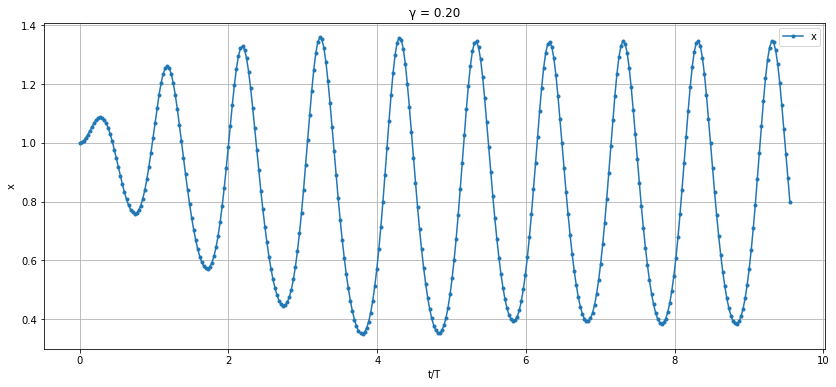
\includegraphics[scale = 0.3]{201.png}
    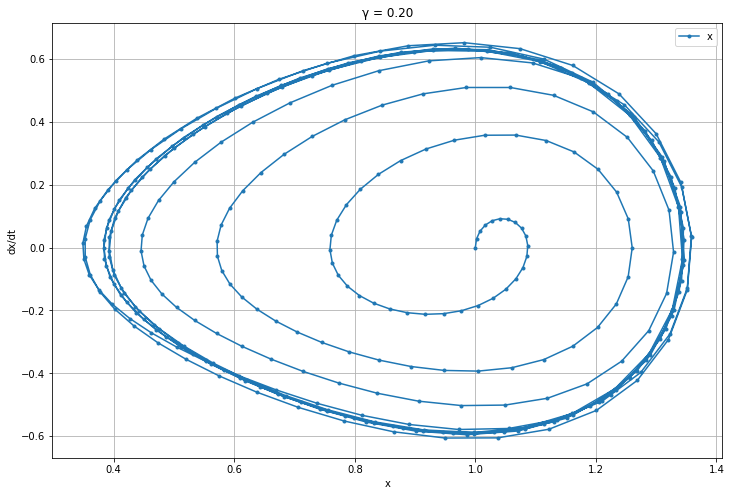
\includegraphics[scale = 0.23]{202.png}
    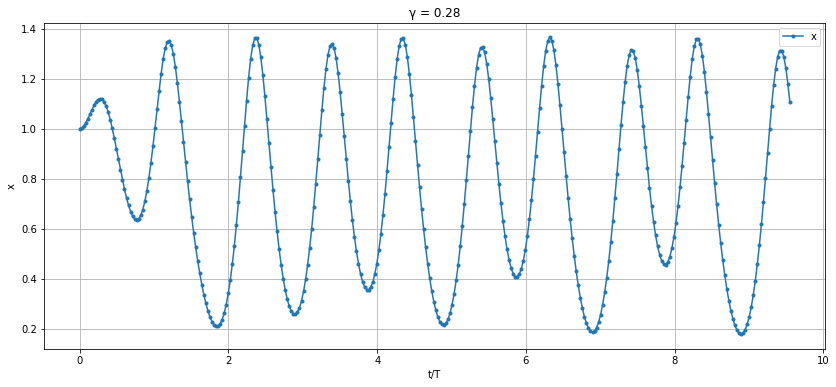
\includegraphics[scale = 0.3]{281.png}
    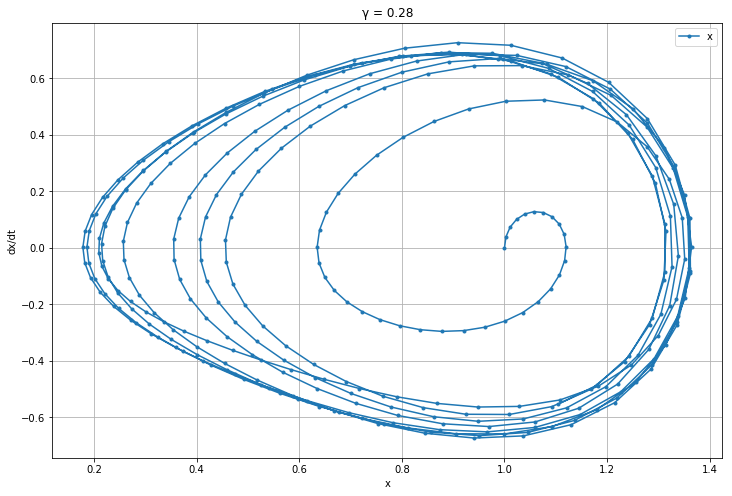
\includegraphics[scale = 0.23]{282.png}
    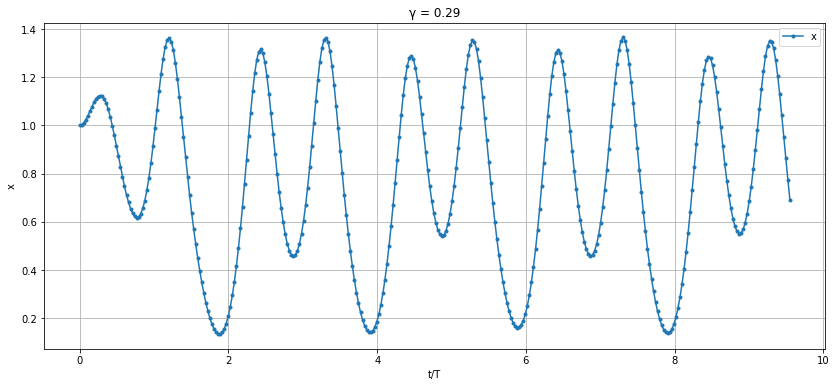
\includegraphics[scale = 0.3]{291.png}
    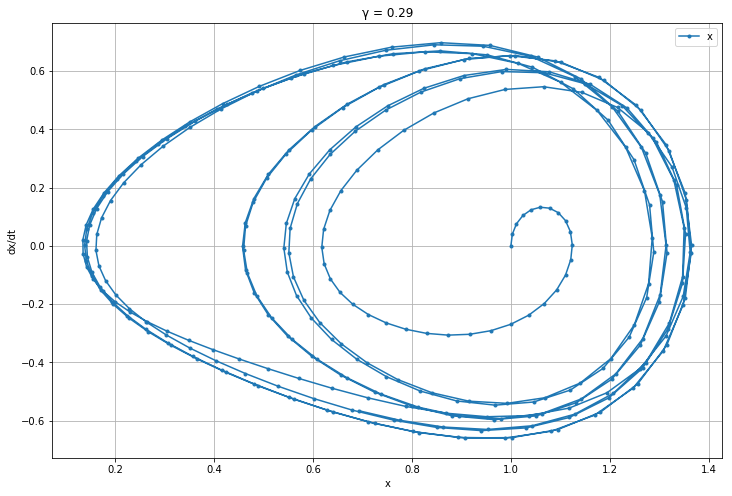
\includegraphics[scale = 0.23]{292.png}
    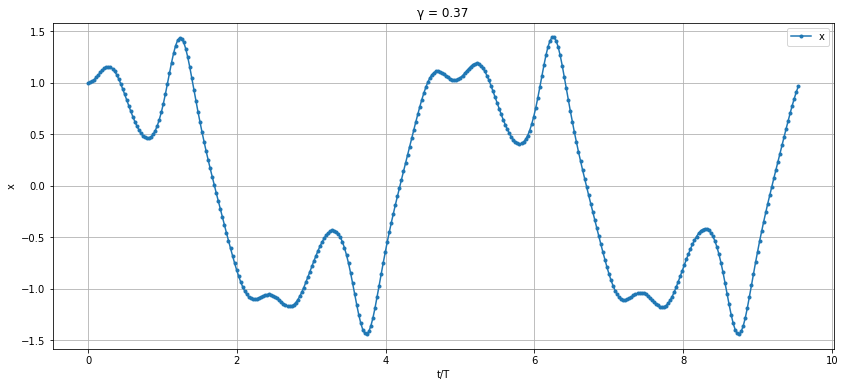
\includegraphics[scale = 0.3]{371.png}
    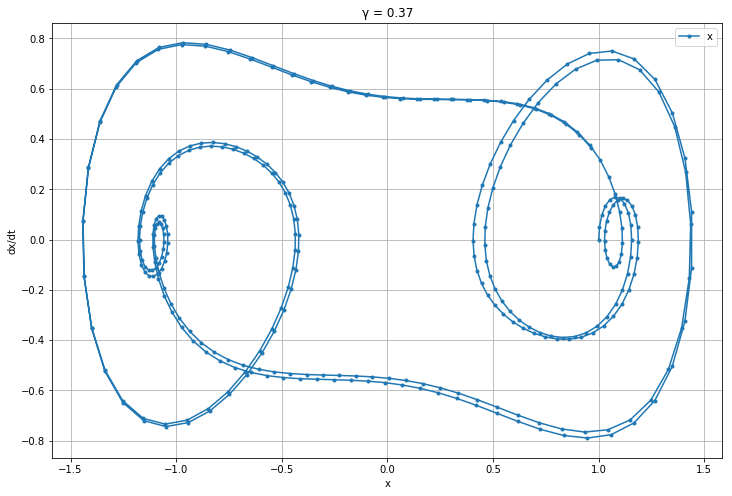
\includegraphics[scale = 0.23]{372.png}
    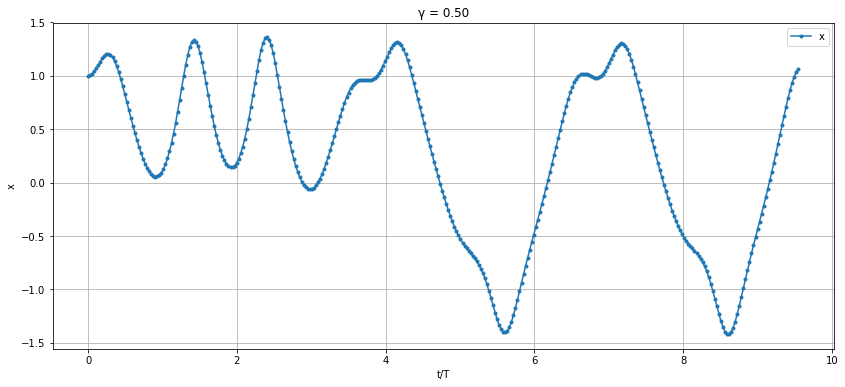
\includegraphics[scale = 0.3]{501.png}
    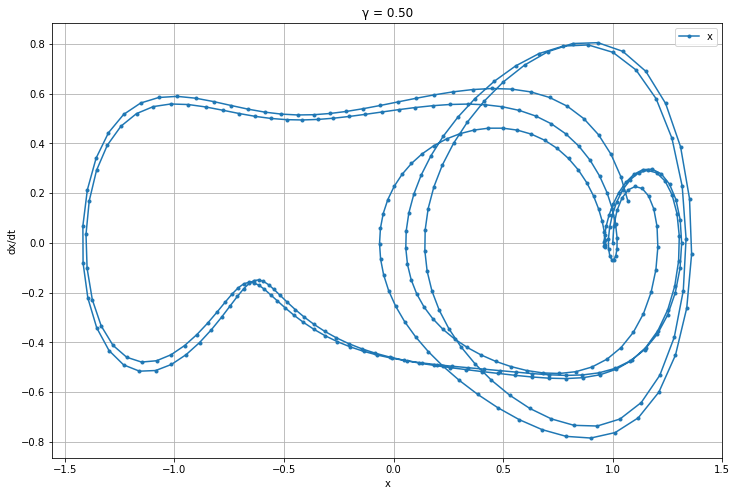
\includegraphics[scale = 0.23]{502.png}
    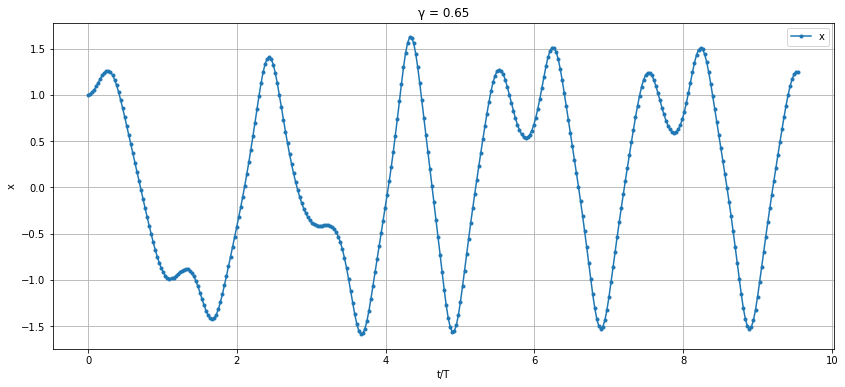
\includegraphics[scale = 0.3]{651.png}
    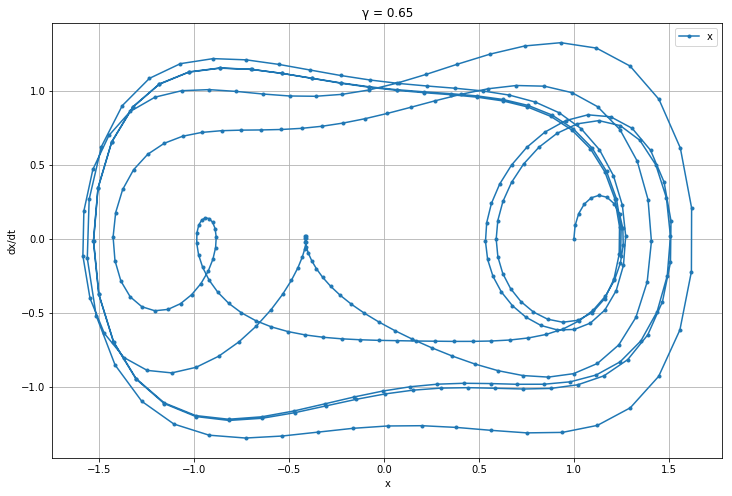
\includegraphics[scale = 0.23]{652.png}
\end{center}

\section{Conclusión}
Pudimos observar que la ecuación de Duffing en estas condiciones, se comporta como un sistema caótico especialmente si modificamos el parámetro de la amplitud de la fuerza impulsora.

\section{Referencias}
\begin{itemize}
    \item Duffing Equation. Consultado de Wikipedia. Sitio web:
    
    https://en.wikipedia.org/wiki/Duffing\_equation
    
    \item Función ode de SciPy. Consultado de SciPy.org. Sitio web:
    
    https://docs.scipy.org/doc/scipy/reference/generated/scipy.integrate.ode.html
    
    \item Función odeint de SciPy. Consultado de SciPy.org. Sitio web:
    
    https://docs.scipy.org/doc/scipy/reference/generated/scipy.integrate.odeint.html
    
    \item A modified phase-fitted Runge–Kutta method for the numerical solution of the Schrödinger equation. Consultado de Journal of Mathematical Chemistry. Sitio web:
    
    https://link.springer.com/content/pdf/10.1023/A:1013185619370.pdf
\end{itemize}

\end{document}
